\chapter{Etude Expérimentale}
\section{Tableau Des Expérimentations}

\par
\resizebox{17cm}{!}{
\begin{tabular}{| c | c | c | c | c | c | c | c | c | c | c | c | c |  }
    \hline
    Nombre de disque (n) & 5 & 10 & 15 & 20 & 25 & 30 & 35 & 40 & 45 & 50 &...& 100   \\
    \hline
    Temps d’exécution (s) &  0.000 & 0.000 & 0.000 & 0.023 & 0.784 & 25.946 & 810.640 & // & // & // & & // \\
    \hline
    Nombre des déplacements effectués &  31 & 1023 & 32767 & 1048575 & 33554431 & 1073741823 & 34359738367 & // & // & // & & //  \\
    \hline
\end{tabular}}

\section{Simulation de la complexité temporelle et spatiale théorique de l’algorithme de résolution}
\subsection{Simulation de la complexité temporelle théorique}
\begin{figure}[H]
    \centering
        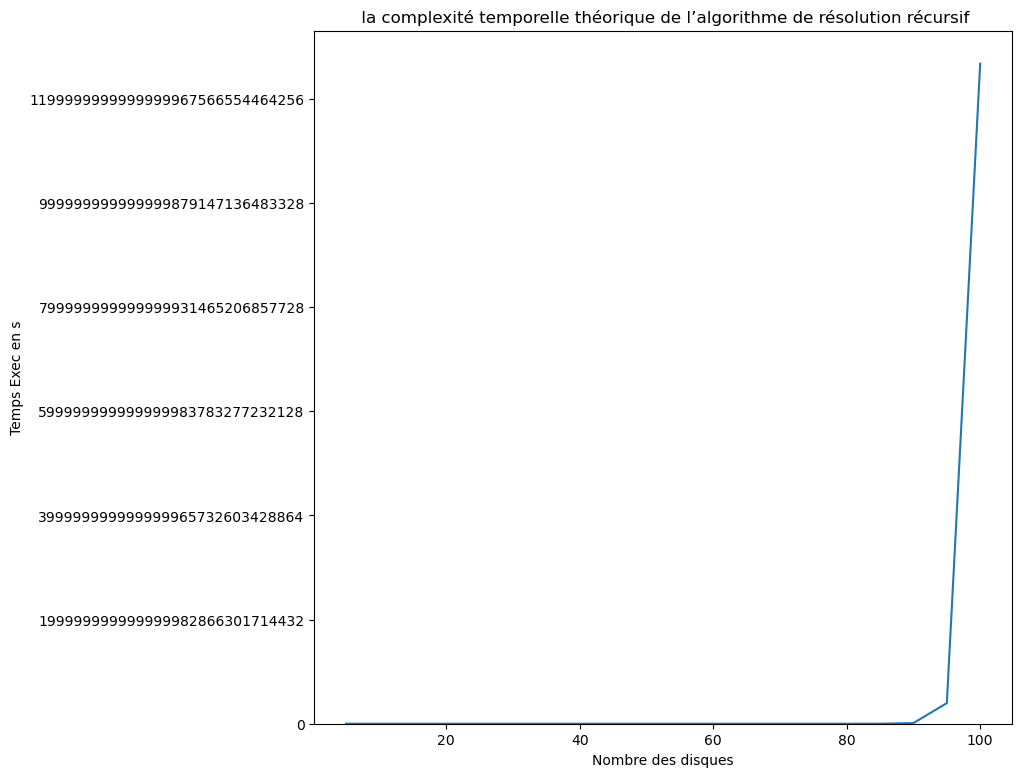
\includegraphics[scale=0.7]{ressources/temporelle.png}
        \caption{{Simulation de la complexité temporelle théorique de l’algorithme de résolution }}
    \label{fig:insertch}
\end{figure}
\par
\subsection{Simulation de la complexité spatiale théorique }
\begin{figure}[H]
    \centering
        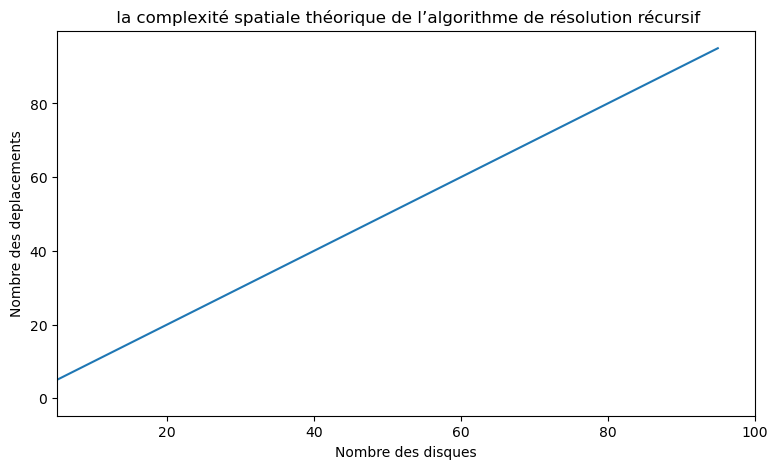
\includegraphics[scale=0.7]{ressources/spatiale.png}
        \caption{{Simulation de la complexité spatiale théorique de l’algorithme de résolution }}
    \label{fig:insertch}
\end{figure}
\par
\section{Le meilleur, moyen et pire cas de l'algorithme de résolution}
\subsection{Le meilleur, moyen et pire cas de la complexite spatiale}
\par Pour chaque appel de la fonction hanoi la solution du problème de taille k est stocké dans une pile et l’espace pri est indépendant de l’appel précédent donc on peut réutiliser l’espace  de 1er appel récursif alors la complexité spatiale de tour d’hanoi est O(n) dans tous les cas.

\subsection{Le meilleur, moyen et pire cas de la complexité temporelle}
\par Le temps pris par un algorithme pour les Tours de Hanoi sera proportionnel au nombre de fois où nous déplaçons un disque car dans ce cas la un mouvement élémentaire consiste à déplacer un disque d'une tige à une autre. 
\par Soit T(n) le nombre minimum de déplacements de disques nécessaires pour résoudre une instance Tours de Hanoi avec n disques. Si n > 1, T(n) est égal à 2 T(n-1) + 1 car nous pouvons d'abord déplacer récursivement les n-1 premiers disques vers la tige auxiliaire, déplacer le plus grand disque vers la tige de destination, puis déplacer récursivement la pile de la tige auxiliaire vers la tige de destination.
\par Le nombre minimum de déplacements de disques dans tous les cas sera toujours le résultat de cette formule récursive et uniquement dépendant du paramètre ‘n’ le nombre des disques  en entré car il n'y a qu'un seul "cas" pour chaque taille d'entrée avec une seule contrainte sur les disques d'être trié suivant un ordre croissant donc  la complexité temporelle dans le meilleur, moyen et pire cas est $O(2^n)$ qui est obtenue par l'élimination de la récursivité comme nous l’avons déjà montré dans la partie II.\\

\section{Analyse des résultats}
\par En observant  les graphes nous remarquons que pour un nombre de disques modéré inférieur à 35  le problème de tour d’hanoi peut être résolu dans un temps d'exécution acceptable qui dépend de la performance de la machine utilisée mais en dépassant  le seuil des 45 le temps d'exécution croît très rapidement lorsque n augmente car  le nombre minimum de déplacements requis pour une instance des Tours de Hanoi avec n disques est de $2^n - 1$ qui correspond à la complexité exponentielle $O(2^n)$.
\par En outre, l’espace requis par l'algorithme de résolution est linéaire ce qui fait que la complexité temporelle est le seul obstacle majeur empêchant d'appliquer cette solution.
\par Pour approximer  l'importance de cette complexité temporelle, supposons qu'il nous faille une seconde pour déplacer un disque d'une tige à une autre tige. Alors, pour résoudre une instance avec 64 disques, il nous faudra environ 585 milliards d'années avec les machines les plus performantes d'aujourd'hui!
